\chapter{Molecular Dynamics}

\section{Estimating statistical error}
With all experiments it is important to have a method of quantifying the statistical error in data, and computer simulations are not exempt.
The measurements made in a molecular dynamics simulation are time-averages of observable and are evaluated over some finite simulation time as
$$A_{\tau} = \frac{1}{\tau} \int_{t=0}^{\tau} A(t) dt.$$
Frenkel and Smit show us that the variance in this average may be calculated as 
$$\sigma^{2}(A) = \frac{1}{\tau^{2}} \int_{0}^{\tau} \int_{0}^{\tau} dt dt' \big \langle [ A(t) - \langle A \rangle ] [A(t') - \langle A \rangle] \big \rangle$$
where the integrand is simply the time-correlation function of fluctations in A\cite{FrenkelSmit}.
In the limit of a simulation time longer than the characteristic decay time $t_{A}^c$ of the correlation function, this error reduces to 
$$\sigma^{2}(A) \approx \frac{2t^{c}_{A}}{\tau}C_{A}(0).$$

This equation demonstrates to us the importance of accounting for correlation between data points in a molecular dynamics simulation. 
The ratio of $\frac{\tau}{t_{A}^{c}}$ gives the number of uncorrelated measurements, and thus it is clear that the variance is inversely proportional to this number.
To estimate the statistical error, one needs only knowledge of the time correlation function of the measured observable.
However, calculating these functions induces significant computational cost.

Despite this, there exist methods for obtaining an estimate of the statistical error and an example of these is block-averaging.
One particular method developed by Flybjerg and Peterson involves applying a blocking transformation to a data set to generate a new uncorrelated data set\cite{Flybjerg}.
They show that the variance of an observable can be estimated as
$$\sigma^{2}(A) \geq \bigg \langle \frac{C_{0}}{n-1} \bigg \rangle$$
where $C_{0}$ is the value of the time-correlation function at $t=0$ and is given by
$$C_{0} \equiv \frac{1}{n} \sum_{k=1}^{n}(A_{k} - \bar{A})(A_{k} - \bar{A}).$$
The key to the analysis is to determine the value of this error by finding the block size at which this estimate reaches a plateau, thus providing a lower bound on the value of $\sigma^{2}(A)$. 

Their method proceeds as follows:
\begin{enumerate}
 \item Take a set of data $\{A_{1},A_{2},...,A_{n}\}$.
 \item Compute $\frac{C_{0}}{n-1}$ and use as an estimator for $\big \langle \frac{C_{0}}{n-1} \big \rangle$.
 \item Apply the block transformation using
	$A_{i}' = \frac{1}{2} (A_{2i-1} + A_{2i}).$
	This halves the size of the data set.
 \item Compute new estimate of error.
 \item Repeat process until $n' = 2$.

Using these data, it is then possible to plot the estimates for $\sigma^{2}(A)$ against the size of the individual blocks.
In doing so, one can obtain a good estimate of the error from the value to which the data plateau.
Their paper also provides an equation for estimating the error in $\sigma^{2}(A)$ which is independent of any assumptions; this is given as
$$\sqrt{\frac{2}{n-1} \times \frac{C_{0}'}{n'-1}}.$$
They note that this method gives the same statistical error as the more theoretically rigorous time-correlation method but with a dramatic decrease in computational cost.

\begin{figure*}
\centering
        \includegraphics[scale=0.65]{block_average_10e6.eps}
	\\
        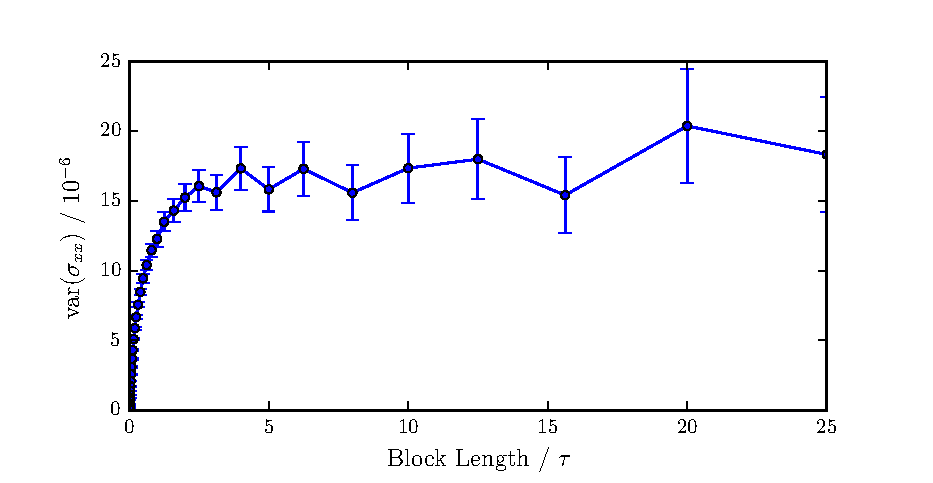
\includegraphics[scale=0.65]{block_average_1e6.eps}
	\caption{The blocking analysis for a simulation time of 10,000,000 timesteps and 1,000,000 timesteps shows clear plateaus in the estimate of the error at block sizes of 10,000 and 5,000 respectively.
This can be used to estimate the size of blocking needed to decorrelate data in the correspinding molecular dynamics simulations.}
\label{blocking}
\end{figure*}

Using a standard binary mixture simulation identical to those used to calculate the Marangoni forces at the interface, a blocking analysis was carried out for a simulation time of $10^{6}$ timesteps and $10^{7}$ timesteps as shown in Fig \ref{blocking}.
These data show a clear plateau at a block size of 10,000 timesteps for the longer simulation time and 5,000 timesteps for the shorter run, with little increase in the error of $\sigma^{2}$ until a much larger block size.
This information can be used to infer a suitable size for block averaging data within a LAMMPS simulation in order to yield sufficient decorrelation of individual samples and a good estimate of the statistical error. 



